\subsubsection{FRI}\label{section: starky-fri}

\begin{figure}[!htp]
    \centering
    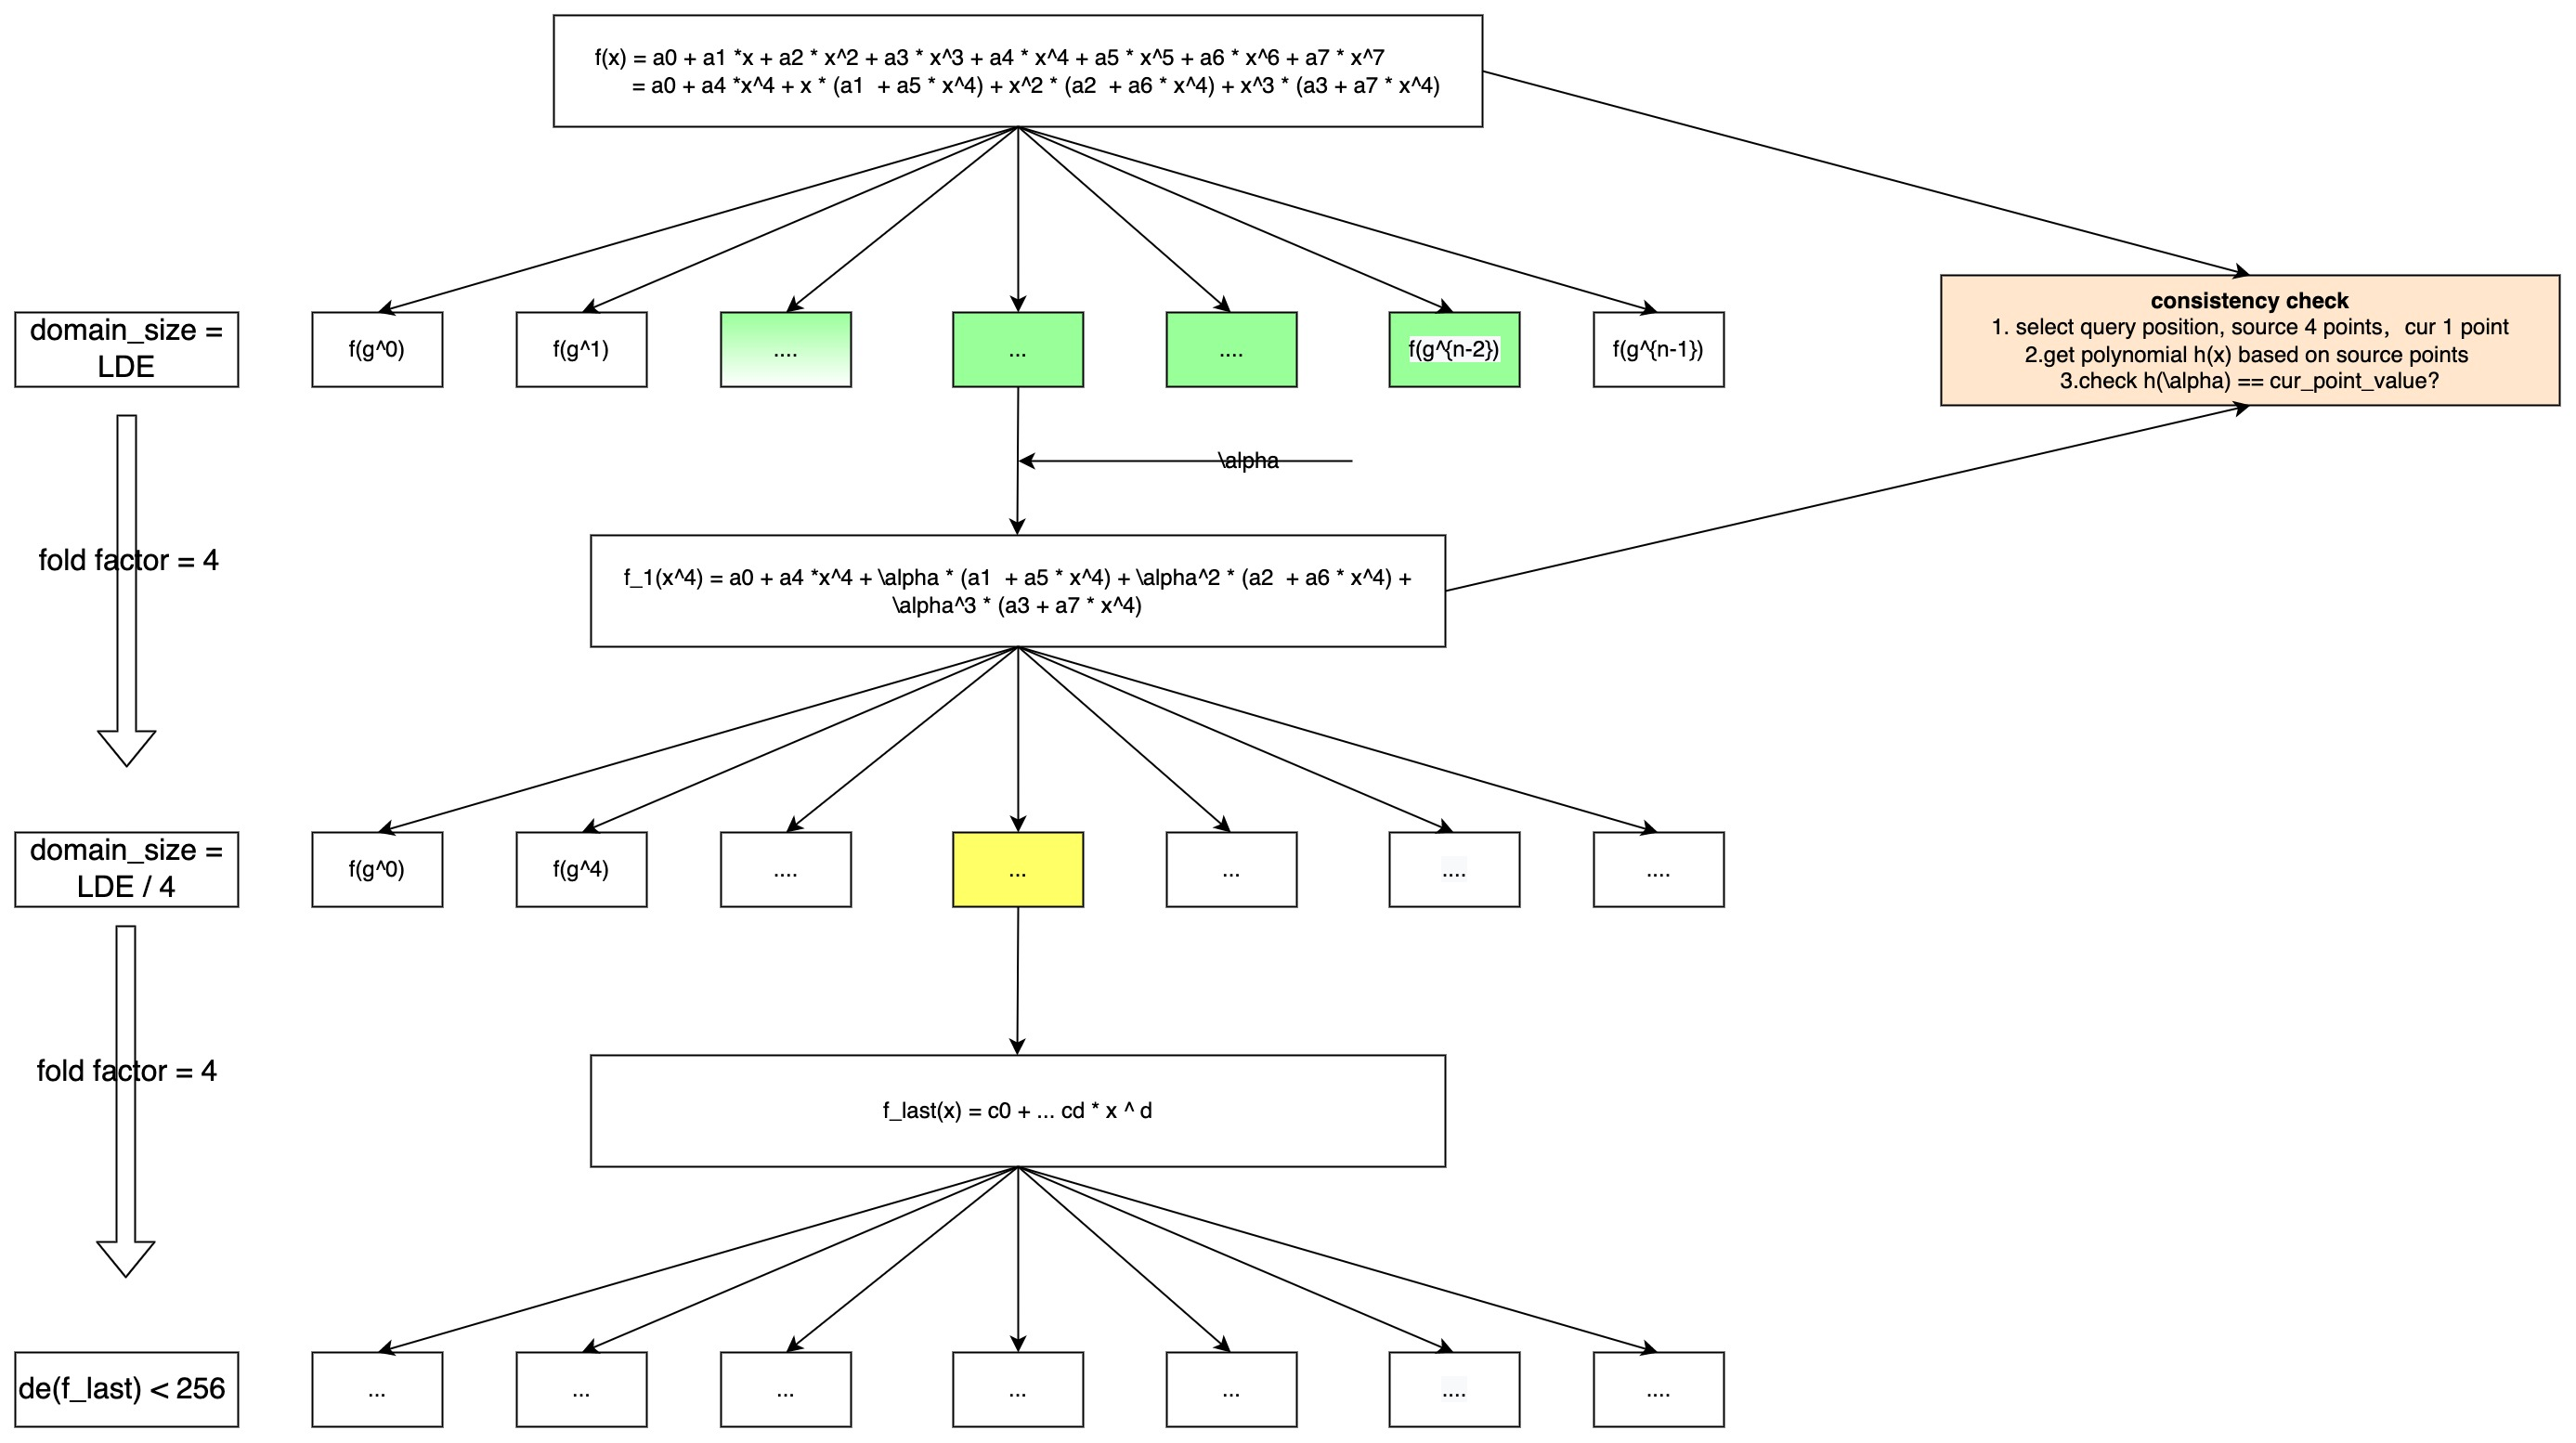
\includegraphics[width=0.8\textwidth]{fri.jpg}
    \caption{FRI}
    \label{fig: FRI}
\end{figure}

FRI is a protocol that establishes that a committed polynomial has a bounded degree. The acronym FRI stands for Fast Reed-Solomon IOP of Proximity, where IOP stands for interactive oracle proof. Ola uses Deep-FRI for its polynomial commitment scheme. Readers can read the \href{https://arxiv.org/abs/1903.12243}{paper} for more details.